% !TeX root = RJwrapper.tex
\title{RTCGA.data - The Family of R Packages with Data from The Cancer Genome
Atlas Study}
\author{by Marcin Kosinski, Przemysław Biecek}

\maketitle

\abstract{
The following article presents RTCGA.data: a family of R packages with
data from The Cancer Genome Atlas Project (TCGA) study. TCGA is a
comprehensive and coordinated effort to accelerate our understanding of
the molecular basis of cancer through the application of genome analysis
technologies, including large-scale genome sequencing {[}1{]}. We
converted selected datasets from this study into few separate packages
that are hosted on one GitHub
repository\footnote{https://github.com/mi2-warsaw/RTCGA.data}. These R
packages make selected datasets easier to access and manage. Data sets
in RTCGA.data packages are large and cover complex relations between
clinical outcomes and genetic background. These packages will be useful
for at least three audiences: biostatisticians that work with cancer
data; researchers that are working on large scale algorithms; teachers
that are presenting data analysis method on real data problems.
}

\section{Motivation}\label{motivation}

The Cancer Genome Atlas (TCGA) Data Portal provides a platform for
researchers to search, download, and analyze data sets generated by
TCGA. It contains clinical information, genomic characterization data,
and high level sequence analysis of the tumor genomes {[}1{]}.

TCGA data is available through Firehose Broad GDAC portal {[}1{]}. One
can select cancer type (cohort) and data type (e.g.~clinical, RNA
expression, methylation, ..) and download a \texttt{tar.gz} file with
compressed data.

When working with many cancer types we find this approach burdensome:

\begin{itemize}
\itemsep1pt\parskip0pt\parsep0pt
\item
  If one requires to download datasets containing e.g.~information about
  genes' expressions for all available cohorts types (TCGA collected
  data for more than 30 various cancer types) one would have to go
  through the click-to-download process many times, which is
  inconvenient and time-consuming.
\item
  Clinical datasets from TCGA project are not in a standard tidy data
  format, which is: one row for one observation and one column for one
  variable. They are transposed which makes work with that data
  burdensome. That becomes more onerous when one would like to
  investigate many clinical datasets.
\item
  Datasets containing information on some data types (e.g.~gene's
  mutations) are not in one easy-to-handle file. Every patient has it's
  own file, what for many potential researchers may be an impassable
  barrier.
\item
  Data governance for many datasets for various cohorts saved in
  different folders with strange (default after untarring) names may be
  exhausting and uncomfortable for researchers that are not very skilled
  in data management or data processing.
\end{itemize}

For these reasons we prepared selected datasets from the TCGA project in
an easy to handle and process way and embed them in 4 separate R
packages. All packages can be installed from BioConductor by evaluating
the following code:

\begin{Schunk}
\begin{Sinput}
source("https://bioconductor.org/biocLite.R")
biocLite("RTCGA.clinical") 
biocLite("RTCGA.rnaseq") 
biocLite("RTCGA.mutations") 
biocLite("RTCGA.cnv") 
\end{Sinput}
\end{Schunk}

\section{Patient's barcode as a key to merge
data}\label{patients-barcode-as-a-key-to-merge-data}

A TCGA barcode is composed of a collection of identifiers. Each
specifically identifies a TCGA data element. An illustration on what
each part of the patient's barcode can be found on \newline ~
\href{https://wiki.nci.nih.gov/display/TCGA/TCGA+barcode}{\url{https://wiki.nci.nih.gov/display/TCGA/TCGA+barcode}}.

\section{How to work with RTCGA.data
family}\label{how-to-work-with-rtcga.data-family}

\pkg{RTCGA.data} family contains 4 packages:

\begin{itemize}
\itemsep1pt\parskip0pt\parsep0pt
\item
  \texttt{RTCGA.clinical} package containing clinical datasets from
  TCGA. Each cohort contains one dataset prepared in a tidy format. Each
  row, marked with patients' barcode, corresponds to one patient.
  Clinical data format is explained here
  \url{https://wiki.nci.nih.gov/display/TCGA/Clinical+Data+Overview}
\item
  \texttt{RTCGA.rnaseq} package containing genes' expressions datasets
  from TCGA. Each cohort contains one dataset with over 20 thousand
  columns corresponding to genes' expression. Rows correspond to
  patients, that can be matched with the patient's barcode. Genes'
  expressions data format is explained here
  \url{https://wiki.nci.nih.gov/display/TCGA/RNASeq+Version+2}
\item
  \texttt{RTCGA.mutations} package containing genes' mutations datsets
  from TCGA. Each cohort contains one dataset with extra column
  specifying patient's barcode which enables to distinguish which rows
  correspond to which patient. Mutations' data format is explained here
  \url{https://wiki.nci.nih.gov/display/TCGA/Mutation+Annotation+Format+(MAF)+Specification}.
\item
  \texttt{RTCGA.cnv} package containing copy number (the number of
  copies of a given gene per cell) variation datasets from TCGA.
\end{itemize}

More detailed information about datasets included in \pkg{RTCGA.data}
family are shown in Table \ref{data_details}

\begin{widetable}[h]
\centering
\caption{\label{data_details}Dimensions of available datasets in \pkg{RTCGA.family}.}
\begin{tabular}{rlllllll}
  \toprule
 & Disease Name & Cohort & Cases & clinical & cnv\footnote{The second dimension is always equal to 6.} & mutations & rnaseq\footnote{The second dimension is always equal to 20532.} \\ 
  \toprule
1 & Adrenocortical carcinoma & ACC & 92 & 92 x 1115 & 21052 & 20255 x 53 & 79 \\ 
  2 & Bladder urothelial carcinoma & BLCA & 412 & 401 x 2098 & 105795 & 39441 x 96 & 427 \\ 
  3 & Breast invasive carcinoma & BRCA & 1098 & 1085 x 3668 & 284510 & 91471 x 68 & 1212 \\ 
  4 & Cervical and endocervical cancers & CESC & 307 & 305 x 1674 & 59450 & 46740 x 58 & 309 \\ 
  5 & Cholangiocarcinoma & CHOL & 36 & 36 x 846 & 7570 & 6789 x 49 & 45 \\ 
  6 & Colon adenocarcinoma & COAD & 460 & 453 x 3149 & 91166 & 62683 x 40 & 328 \\ 
  7 & Colorectal adenocarcinoma & COADREAD & 631 & 624 x 3488 & 126931 &  &  \\ 
  8 & Lymphoid Neoplasm Diffuse Large... & DLBC & 58 & 47 x 760 & 9343 &  & 28 \\ 
  9 & Esophageal carcinoma & ESCA & 185 & 183 x 1197 & 60803 &  & 196 \\ 
  10 & FFPE Pilot Phase II & FPPP & 38 & 38 x 3277 &  &  &  \\ 
  11 & Glioblastoma multiforme & GBM & 613 & 593 x 5379 & 146852 & 22362 x 80 & 166 \\ 
  12 & Glioma & GBMLGG & 1129 & 1085 x 5660 & 226643 &  &  \\ 
  13 & Head and Neck squamous cell carcinoma & HNSC & 528 & 523 x 1754 & 110289 & 52077 x 90 & 566 \\ 
  14 & Kidney Chromophobe & KICH & 113 & 111 x 907 & 10164 & 7624 x 37 & 91 \\ 
  15 & Pan-kidney cohort (KICH+KIRC+KIRP) & KIPAN & 973 & 917 x 2766 & 142122 & 73527 x 36 & 1020 \\ 
  16 & Kidney renal clear cell carcinoma & KIRC & 537 & 533 x 2682 & 85044 & 26785 x 36 & 606 \\ 
  17 & Kidney renal papillary cell carcinoma & KIRP & 323 & 273 x 1890 & 46914 & 15745 x 53 & 323 \\ 
  18 & Acute Myeloid Leukemia & LAML & 200 & 200 x 1148 & 28324 & 2781 x 65 & 173 \\ 
  19 & Brain Lower Grade Glioma & LGG & 516 & 492 x 2127 & 79791 & 10170 x 39 & 530 \\ 
  20 & Liver hepatocellular carcinoma & LIHC & 377 & 364 x 1583 & 93328 & 28089 x 49 & 423 \\ 
  21 & Lung adenocarcinoma & LUAD & 585 & 521 x 3009 & 122927 & 72770 x 92 & 576 \\ 
  22 & Lung squamous cell carcinoma & LUSC & 504 & 495 x 2692 & 134864 & 65482 x 87 & 552 \\ 
  23 & Mesothelioma & MESO & 87 & 87 x 893 & 18335 &  & 86 \\ 
  24 & Ovarian serous cystadenocarcinoma & OV & 602 & 591 x 3626 & 261680 & 20534 x 44 & 265 \\ 
  25 & Pancreatic adenocarcinoma & PAAD & 185 & 185 x 1248 & 34808 & 15779 x 85 & 183 \\ 
  26 & Pheochromocytoma and Paraganglioma & PCPG & 179 & 179 x 1186 & 31256 & 4784 x 91 & 187 \\ 
  27 & Prostate adenocarcinoma & PRAD & 499 &  & 117345 & 12679 x 86 & 550 \\ 
  28 & Rectum adenocarcinoma & READ & 171 & 171 x 2740 & 35765 & 22143 x 40 & 105 \\ 
  29 & Sarcoma & SARC & 260 &  & 106617 & 26753 x 78 &  \\ 
  30 & Skin Cutaneous Melanoma & SKCM & 470 & 469 x 1875 & 108084 & 276271 x 91 & 472 \\ 
  31 & Stomach adenocarcinoma & STAD & 443 & 443 x 1690 & 118389 & 148808 x 80 &  \\ 
  32 & Stomach and Esophageal carcinoma & STES & 628 & 626 x 1828 & 179192 & 148808 x 80 & 196 \\ 
  33 & Testicular Germ Cell Tumors & TGCT & 150 & 134 x 983 & 24952 & 14826 x 58 & 156 \\ 
  34 & Thyroid carcinoma & THCA & 503 & 502 x 1662 & 55377 & 7862 x 91 & 568 \\ 
  35 & Thymoma & THYM & 124 & 123 x 848 & 15571 &  & 122 \\ 
  36 & Uterine Corpus Endometrial Carcinoma & UCEC & 560 & 540 x 2180 & 127430 & 185108 x 50 & 201 \\ 
  37 & Uterine Carcinosarcoma & UCS & 57 & 57 x 918 & 19298 & 11210 x 91 & 57 \\ 
  38 & Uveal Melanoma & UVM & 80 & 80 x 594 & 12973 & 2607 x 91 & 80 \\
   \bottomrule
\end{tabular}
\end{widetable}

After installation, one can load any package from \pkg{RTCGA.data}
family with commands

\begin{Schunk}
\begin{Sinput}
library(RTCGA.clinical)
library(RTCGA.rnaseq)
library(RTCGA.mutations)
library(RTCGA.cnv)
\end{Sinput}
\end{Schunk}

and one can check what datasets are available (Table \ref{data_details})
with commands

\begin{Schunk}
\begin{Sinput}
?clinical
?rnaseq
?mutations
?cnv
\end{Sinput}
\end{Schunk}

The data loading proceeds in a regular way. Simply type

\begin{Schunk}
\begin{Sinput}
data(cohort.package)
\end{Sinput}
\end{Schunk}

where \texttt{cohort} corresponds to a specific Cohort of patients and
\texttt{package} corresponds to the one of four packages from
\pkg{RTCGA.data} family.

\newpage

\section{Examples of applications}\label{examples-of-applications}

\subsection{The Kaplan-Meier estimate of the survival curves with the
clinical
data}\label{the-kaplan-meier-estimate-of-the-survival-curves-with-the-clinical-data}

\pkg{RTCGA.data} family is excellent when one researches in a field of
survival analysis and genomics. Survival times for patients are included
in clinical datasets. The following example plots Kaplan-Meier {[}5{]}
estimates of the survival functions for patients suffering from LUAD
cancer, divided into stages of the cancer.

\begin{Schunk}
\begin{Sinput}
library(dplyr)
library(RTCGA.clinical)
#library(devtools);biocLite("mi2-warsaw/RTCGA.tools") 
library(RTCGA.tools)
library(survival)
library(survMisc)

LUAD.clinical %>%
   mutate(
      patient.vital_status = ifelse(LUAD.clinical$patient.vital_status %>% as.character() =="dead",1,0),
      barcode = patient.bcr_patient_barcode %>% as.character(),
      times = ifelse( !is.na(patient.days_to_last_followup),
                 patient.days_to_last_followup %>% as.character() %>% as.numeric(),
                 patient.days_to_death %>% as.character() %>% as.numeric() ),
      stage = RTCGA.tools::mergeStages(LUAD.clinical$patient.stage_event.pathologic_stage)
   ) %>%
   rename(
      therapy = patient.drugs.drug.therapy_types.therapy_type
   ) %>%
   filter( !is.na(times) ) -> LUAD.clinical.selected 

LUAD.clinical.selected %>%
   survfit( Surv(times, patient.vital_status) ~ stage, data = .) %>%
   survMisc:::autoplot.survfit( titleSize=12, type="CI" ) %>%
   .[[2]] -> km_plot_luad
\end{Sinput}
\end{Schunk}

\begin{Schunk}
\begin{Soutput}
pdf 
  2 
\end{Soutput}
\end{Schunk}

\begin{figure}[h!]
\begin{centering}
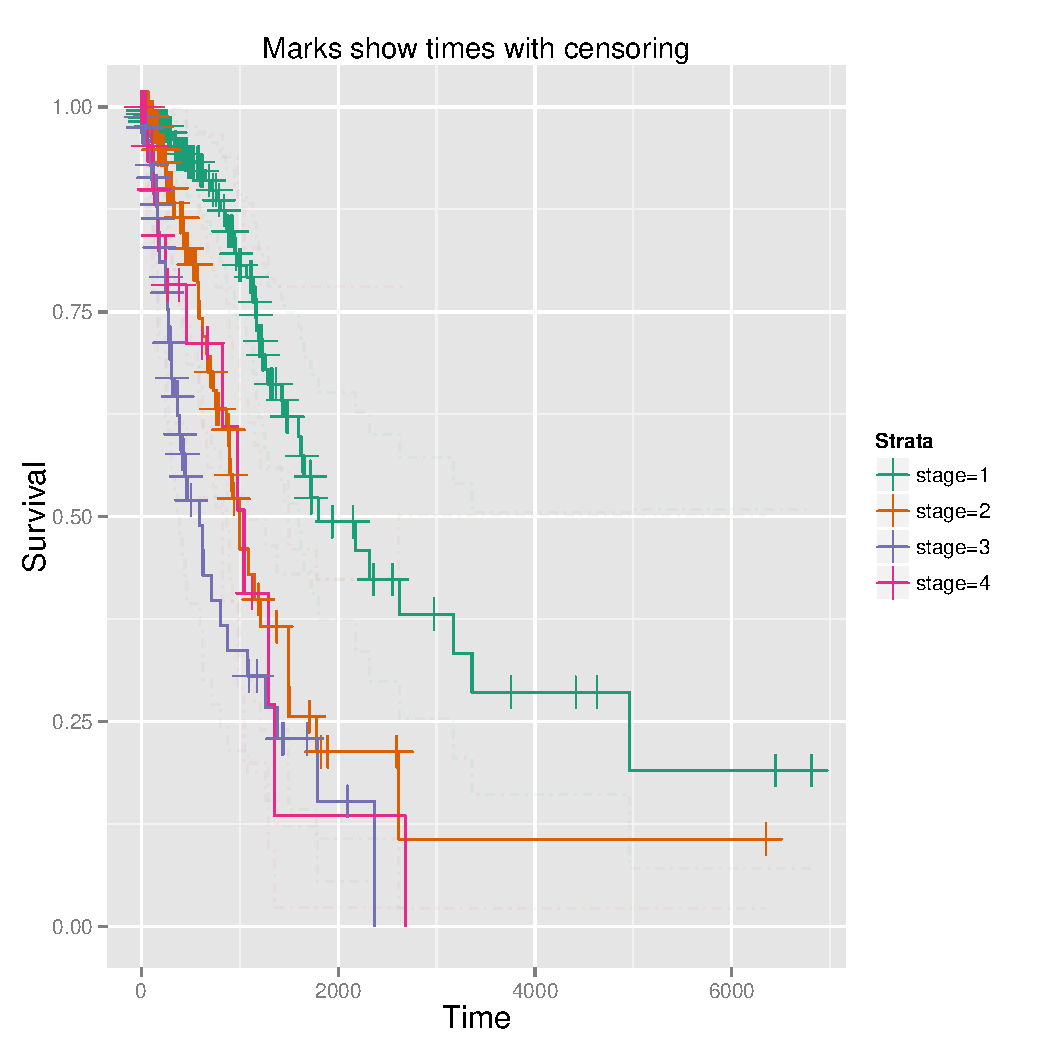
\includegraphics[width=12cm, height=8cm]{km_plot_luad.pdf}
\caption{\label{km_plot}The Kaplan-Meier estimate of the survival curve for the LUAD cancer. }
\end{centering}
\end{figure}

\newpage

\subsection{The Cox proportional hazards model with the genes' mutations
data}\label{the-cox-proportional-hazards-model-with-the-genes-mutations-data}

In a simple way one can use previously selected data to merge them with
genes' mutations data and to compute Cox proportional hazards model
{[}9{]}. Moreover, the goodness of fit can be checked with the plot of
Martingale Residuals - Figure \ref{figRes}.

\begin{Schunk}
\begin{Sinput}
library(RTCGA.mutations)
library(ggthemes)
LUAD.clinical.selected %>%
      left_join( y = LUAD.mutations %>%
                    filter( Hugo_Symbol == "TP53") %>%
                    mutate( barcode = barcode %>% as.character %>% tolower %>% substr(1,12) ) %>%
                    select( barcode, Variant_Classification),
                 by = "barcode") %>%
                    mutate( Variant_Classification = divideTP53(Variant_Classification) ) ->
   LUAD.clinical.mutations.selected

(coxph(Surv(times, patient.vital_status)~ as.factor(stage)+Variant_Classification,
      data = LUAD.clinical.mutations.selected) -> LUAD.coxph)
\end{Sinput}
\begin{Soutput}
Call:
coxph(formula = Surv(times, patient.vital_status) ~ as.factor(stage) + 
    Variant_Classification, data = LUAD.clinical.mutations.selected)


                               coef exp(coef) se(coef)     z       p
as.factor(stage)2            0.8072    2.2417   0.2328  3.47 0.00053
as.factor(stage)3            1.3804    3.9764   0.2339  5.90 3.6e-09
as.factor(stage)4            1.1555    3.1756   0.3414  3.38 0.00071
Variant_ClassificationOther  0.4397    1.5523   0.3284  1.34 0.18058
Variant_ClassificationWILD  -0.0365    0.9642   0.2396 -0.15 0.87890

Likelihood ratio test=45.1  on 5 df, p=1.36e-08
n= 508, number of events= 126 
   (2 observations deleted due to missingness)
\end{Soutput}
\end{Schunk}

\begin{Schunk}
\begin{Sinput}
qplot(predict(LUAD.coxph, type="lp"),residuals(LUAD.coxph))+
   theme_tufte(base_size=20)+
   xlab("Linear combinations")+
   ylab("Martingale residuals")+
   geom_hline(yintercept=0, col ="orange", size = 3)
dev.off()
\end{Sinput}
\end{Schunk}

\begin{figure}[h!]
\begin{centering}
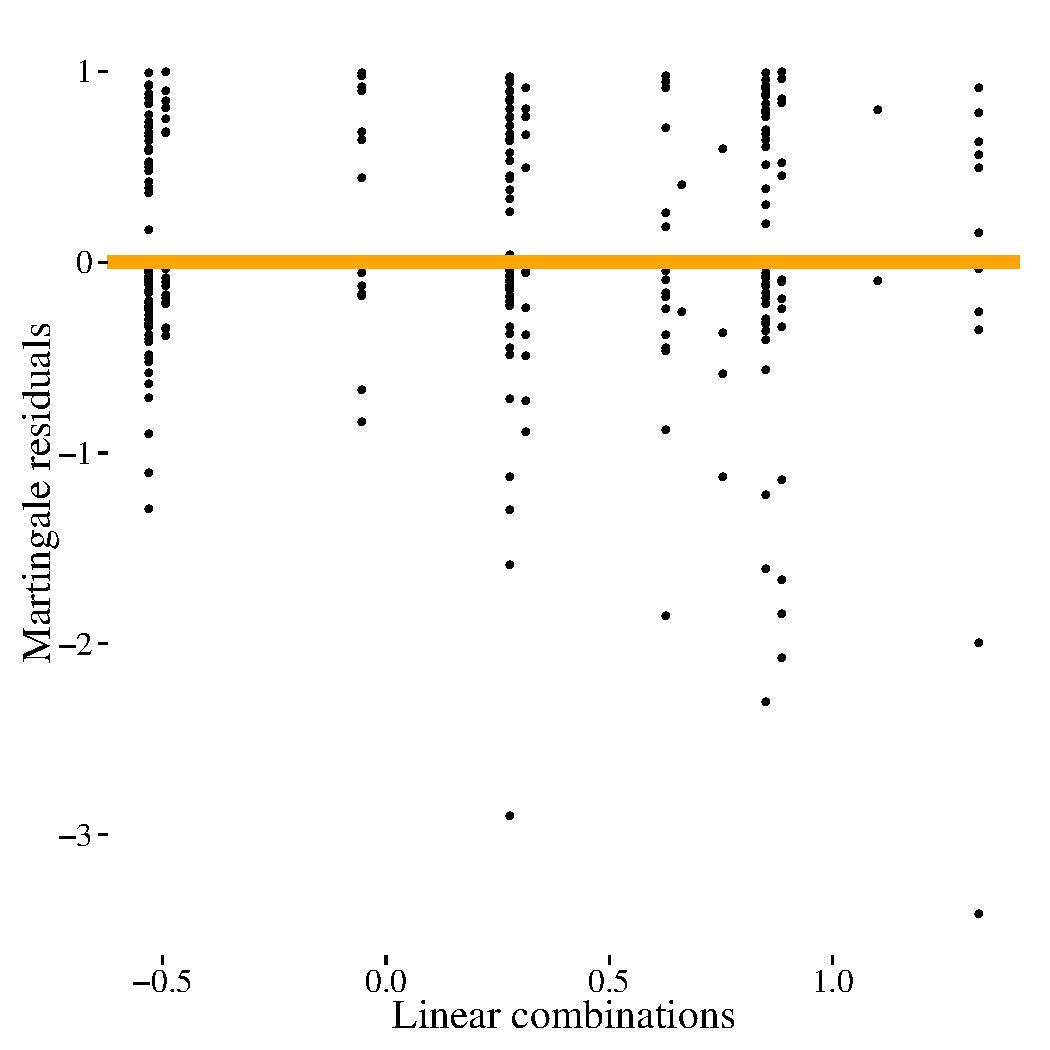
\includegraphics[width=8cm, height=6cm]{res_lp_mart.pdf}
\caption{\label{figRes}Martingale residuals vs. linear combination of the independent variables for the LUAD cancer's Cox proportional hazard model. }
\end{centering}
\end{figure}

\newpage

\subsection{The Principal Components Analysis for the rnaseq
data}\label{the-principal-components-analysis-for-the-rnaseq-data}

One can also perform a Principal Components Analysis, after binding
rnaseq data for few random cancer types like below. It can be seen that
genes' expressions amongs those cancers vary and samples group in view
of cancer type.

\begin{Schunk}
\begin{Sinput}
rbind(ACC.rnaseq, CHOL.rnaseq, GBM.rnaseq, PCPG.rnaseq, UVM.rnaseq) -> rnaseq_sample
# which columns contain only zeros
rnaseq_sample[,-1] %>% colSums() -> rnaseq_col_sums
which(rnaseq_col_sums == 0) -> columns_with_only0
# pca
rnaseq_sample[, -c(1,columns_with_only0+1)] %>%
   prcomp( scale = TRUE ) -> PCA
# labels for pca
lapply(list(ACC.rnaseq, CHOL.rnaseq, GBM.rnaseq, PCPG.rnaseq, UVM.rnaseq), nrow) -> rnaseq_nrow
mapply(rep, 
       c("ACC.rnaseq", "CHOL.rnaseq", "GBM.rnaseq", "PCPG.rnaseq", "UVM.rnaseq"), 
       rnaseq_nrow) %>%
   unlist -> rnaseq_pca_labels
# biplot
#library(devtools);install_github("vqv/ggbiplot")
library(ggbiplot)
rownames(PCA$rotation) <- 1:nrow(PCA$rotation)
ggbiplot(PCA, obs.scale = 1, var.scale = 1,
  groups = rnaseq_pca_labels, ellipse = TRUE, circle = TRUE, var.axes=FALSE) +
  theme(legend.direction = 'horizontal', legend.position = 'top') -> biplot_rnaseq
\end{Sinput}
\end{Schunk}

\begin{figure}[h!]
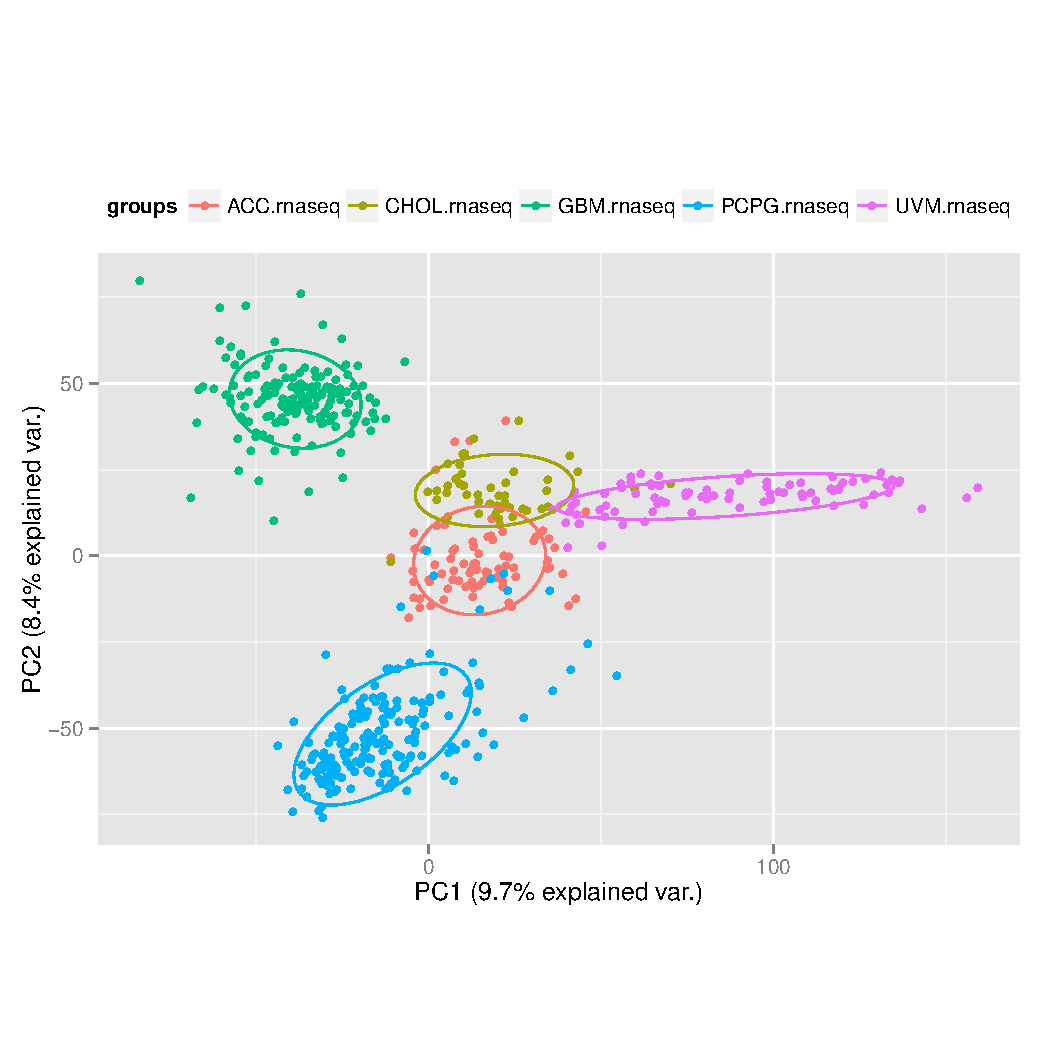
\includegraphics[width=12cm]{biplot_rnaseq.pdf}
\caption{\label{biplot2}The biplot for 2 main components of the principal component analysis of genes' expressions data for 5 various cancer types.}
\end{figure}

\newpage

\begin{Schunk}
\begin{Sinput}
[1] http://cancergenome.nih.gov/

[2] http://gdac.broadinstitute.org/
   
[3] http://cran.r-project.org/bin/windows/Rtools/
   
[4] https://wiki.nci.nih.gov/display/TCGA/TCGA+barcode

[9] Cox D. R., (1972) \textit{Regression models and life-tables (with discussion)}, Journal of the Royal Statistical Society Series B 34:187-220.      
      
[5]  Kaplan, E. L.; Meier, P. (1958). "Nonparametric estimation from incomplete observations". J. Amer. Statist. Assn. 53 (282): 457–481. JSTOR 2281868.

\bibliography{RJreferences}
\end{Sinput}
\end{Schunk}

\address{
Marcin Kosinski\\
Warsaw University of Technology\\
Faculty of Mathematics and Information Science\\ Koszykowa 75, 00-662 Warsaw, Poland\\
}
\href{mailto:M.P.Kosinski@gmail.com}{\nolinkurl{M.P.Kosinski@gmail.com}}

\address{
Przemysław Biecek\\
University of Warsaw\\
Faculty of Mathematics, Informatics, and Mechanics\\ Banacha 2, 02-097 Warsaw, Poland\\
}
\href{mailto:Przemyslaw.Biecek@gmail.com}{\nolinkurl{Przemyslaw.Biecek@gmail.com}}

